% Niveau :      PCSI *
% Discipline :  Chimie Orga I
% Mots clés :   Spectrométrie UV-visible, Réactions acidobasiques

\begin{exercise}{Dureté de l'eau}{2}{PCSI}
{Chimie générale,Réactions de complexation,Dosage,Titrage}{bermu}

\noindent\begin{minipage}{\linewidth}
\begin{wrapfigure}{R}{0.35\textwidth}
    \chemfig{N(-[4]-[-6]^\ominus OOC)(-[-4]-[-6]^\ominus OOC)-[0]-[-2]-[0]N(-[-2]-[0]COO^\ominus)(-[2]-[0]COO^\ominus)}
\end{wrapfigure}

\quad L'EDTA (strucutre ci-contre), noté Y$^{4-}$, est un ligand organique hexadentate très utilisé en chimie minérale pour doser les ions métalliques avec lesquels il a une très bonne affinité par chélation, notamment afin de mesurer la \emph{dureté de l'eau} (la concentration en minéraux de l'eau) par dosage complexométrique.
\end{minipage}

\begin{questions}
\questioncours Influence de la nature du ligand et du métal sur la stabilité du complexe~formé. \\
On prendra pour exemple les complexes EDTA-métal et on commentera la figure suivante : \vspace{-1em}

\begin{EnvUplevel}
    \begin{figure}[H]
        \centering
        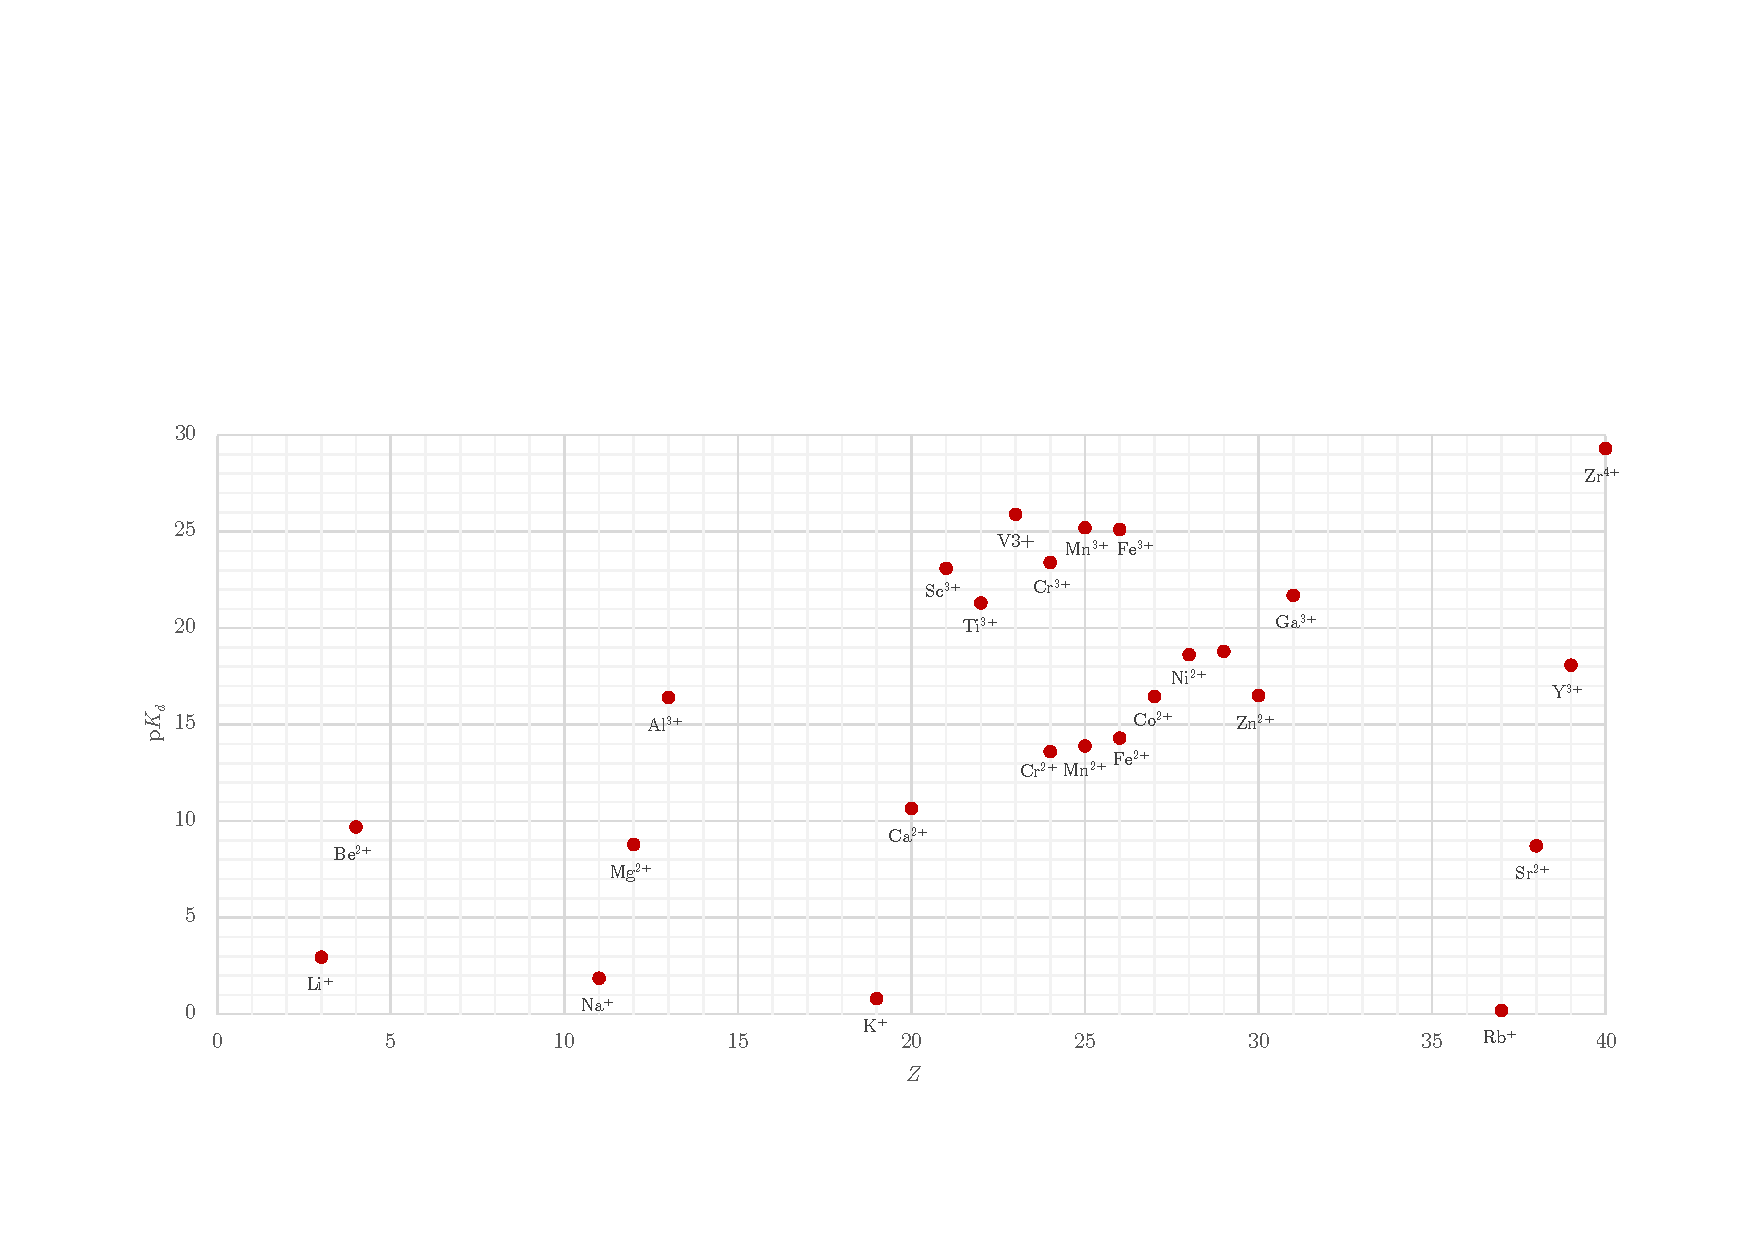
\includegraphics[width=\linewidth]{chimiePC/gene/EDTA.pdf}
        \caption{Constante de dissociation p$K_d$ des complexes métal-EDTA en fonction du numéro atomique $Z$ des ions métalliques.}
    \end{figure}
\end{EnvUplevel}

\question Repérer les sites ligands de Y$^{4-}$ et décrire la structure et la géométrie des complexes chélatés qu'il forme avec les ions métalliques.

\uplevel{On se propose de doser la dureté d'un volume $v_0$ d'eau du robinet avec une solution d'EDTA de concentration $c_1$. On note M$^{n+}$ les ions métalliques susceptibles de réagir.}

\question \'Ecrire la réaction du dosage et indiquer la constante de réaction. \\
Peut-on considérer que la réaction est totale ?

\question Donner la définition de l'équivalence et donner l'expression du volume équivalent $v_\text{eq}$.

\uplevel{Afin de détecter expérimentalement cette équivalence, les complexes d'EDTA étant incolores, on ajoute dans la solution avant le titrage quelques gouttes d'une solution de noir ériochrome T (NET) qui est noire sous sa forme déprotonée Net$^-$ et forme un complexe rouge avec les ions magnésium, calcium environ dix fois moins stables que ceux de l'EDTA.}

\question Décrire l'évolution de la couleur de la solution au cours du titrage.

\question Donner l'expression de la concentration $c_2$ en NET à apporter dans la solution initiale pour que le virage se produise à l’équivalence.

\question En quoi la précision du titrage serait-elle affectée si on introduisait au début du titrage une concentration 10 fois plus importante de NET ? 10 fois moins ? Commenter.

\question{\sffamily Question ouverte :} \'Etablir un protocole expérimental détaillé et chiffré pour mesurer la dureté de l'eau du robinet.

\end{questions}

\paragraph{Données : }~\\
La minéralisation typique de l'eau du robinet en alcalino-terreux est de 10 mg$\cdot$L$^{-1}$.

\noindent Masses molaires (g$\cdot$mol$^{-1}$) : Mg = 24, Ca = 40. 

\end{exercise}

\begin{solution}
\begin{questions}
    \questioncours Dans le cas particulier de l'EDTA, hexadentate :
    \begin{itemize}
        \item On remarque que les complexes des alcalins (colonne 1) sont moins stables que les complexes des alcalino-terreux (colonne 2) eux-mêmes moins stables que les complexes des métaux de transition des colonnes 3 et 4 :
        $$\mathrm{Li^+, Na^+, K^+, Rb^+ < Be^{2+}, Mg^{2+}, Ca^{2+}, Sr^{2+} < Al^{3+}, Sc^{3+}, Y^{3+} < Zr^{4+}.}$$
        
        Globalement, le complexe est plus stable avec des métaux présentant plus de trous dans leur couche de valence car ils forment plus de liaisons de coordination avec les différents sites de l'EDTA.
        
        \item Dans une même colonne, les complexes sont moins stables quand ils sont avec des métaux de rayon ionique élevé car les liaisons sont plus tendues :
        $$\mathrm{Li^+ > Na^+ > K^+ > Rb^+.}$$
        
        \item Pour les métaux de transition, une étude de leur configuration électronique permet de montrer que les plus stables sont ceux qui peuvent accepter 6 électrons en comblant leur couche de valence.
        
        \end{itemize}
    
    \question Les 6 sites ligands de Y$^{4-}$ sont les deux doublets non liants des deux azotes $\overline{\text{N}}$ et les 4 carboxylates COO$^\ominus$.
    
    Ils forment donc des complexes octaèdriques dans lesquels les métaux sont 'mis en cage' par l'EDTA, ce qui favorise grandement la stabilité du complexe.
    
    \question $\mathrm{Y^{4-} + M^{n+} \leftrightharpoons [YM]^{n-4}}$ de constante $1/K_d$ qui est de l'ordre de $10^9 \gg 1$ pour le magnésium : la réaction peut donc être considérée comme totale.
    
    \question L’équivalence est obtenue lorsqu’on a apporté Y$^{4-}$ et M$^{n+}$ dans les proportions st{\oe}chiométriques de la réaction de titrage, ici 1:1, soit
    $$n_\text{eq} = n_\mathrm{Y^{4-}} = n_\mathrm{M^{n+}} \qquad \Longleftrightarrow \qquad v_0 c_0 = c_1 v_\text{eq},$$
    en notant $c_0 = \mathrm{[M^{n+}]}_0$ la \emph{dureté} de l'eau.
    
    \question Au début, l'ion Net$^{-}$ se complexe immédiatement avec les ions métalliques M$^{n+}$ et forme un complexe rouge :
    $$\mathrm{Net^{-} + M^{n+} \longrightarrow MNet^{n-1}}\qquad\text{de constante } K_{d,\textsc{net}} \simeq 10 \times K_d.$$
    \`A l'équivalence, M$^{n+}$ est totalement consommé et la solution redevient noire.
    
    \question Le virage de l'indicateur se produit lorsque $\mathrm{[Net^{-}] \geqslant [MNet^{n-1}]}$, soit pour
    $$K_{d,\textsc{net}} = \mathrm{\dfrac{[Net^{-}][M^{n+}]}{[MNet^{n-1}]}} \geqslant \mathrm{[M^{n+}]_{eq}} \qqtext{soit} \mathrm{[M^{n+}]_{eq}} \leqslant 10^{-8}\text{ M},$$
    indépendemment de $c_2$.
    
    $c_2$ doit donc être simplement très petit devant $c_1$ pour ne pas perturber l'équivalence.
    
    %\`A l’équivalence le titrant a consommé exactement le titré : la réaction est quasi-totale. Il ne reste donc qu'une trace d'ions Y$^{4-}$ et M$^{n+}$, notée $\varepsilon$ telle que :
    %$$K_d = \mathrm{\dfrac{[M^{n+}][Y^{4-}]}{[MY^{n-4}]}} \simeq \dfrac{\varepsilon^2}{\frac{c_0 v_0}{v_0 + v_{eq}}} = \varepsilon^2 \dfrac{1 + c_1/c_0}{c_0} \qquad \Longleftrightarrow \varepsilon = \sqrt{\dfrac{K_d c_0}{1 + c_1/c_0}} \simeq 10^{-6} \text{ M},$$
    %en prenant $c_0 \simeq c_1 \simeq 1$ mM (cf. données) et $K_d \simeq 10^{-9}$.
    
    %Or 
    
    \question Si on apporte 10 plus de fois de NET, la réaction de complexation du NET, qui est quantitative, va déplacer l'équivalence vers de plus faibles volumes.
    
    En revanche, une plus petite concentration laisse inchangée l'équivalence : en revanche on risque de ne plus voir l'indicateur, ce qui serait dommage...
    
    \question{\sffamily Protocole : } d'après les données, $c_0 \simeq 1$ mM. Ainsi, il faut pour un $v_\text{eq} \simeq 20$ mL que $c_1 \simeq 5\times 10^{-4}$~M.
    
    Ensuite, on introduit dans un erlenmeyer $v_0 = 10$ mL d'eau du robinet à l'aide d'une pipette jaugée, une goutte de NET, on dilue jusqu'environ 100 mL pour le la dilution soit négligeable. Dans la burette on introduit une solution d'EDTA à $5\times 10^{-4}$ M préparée avec une fiole jaugée.
    
    \emph{ect.}
    
\end{questions}
\end{solution}